A seguir descrevemos detalhes da implementação do \textit{TOSThread}. Mostraremos a organização dos diretório e os
códigos fonte mais importantes.

\paragraph{Organização dos diretórios:}
O diretório raiz do \textit{TOSThread} é \textit{/opt/tinyos-2.1.1/tos/lib/tosthreads/}.
Abaixo descrevo sua estrutura básica de diretórios e as respectivas descrições\footnote{Todos os arquivos serão referenciados a partir do diretório
raiz \textit{/opt/tinyos-2.1.1/tos/lib/tosthreads/}. i.e. \textit{types/thread.h}}:
\begin{description}
\setlength{\itemsep}{0.2pt}
\setlength{\parskip}{0pt}
\setlength{\parsep}{0pt}
    \item[chips:] Código específico de chips.
    \item[interfaces:] Interfaces do sistema.
    \item[lib:] Extensões e subsistemas.
        \begin{description}
        \setlength{\itemsep}{0.2pt}
        \setlength{\parskip}{0pt}
        \setlength{\parsep}{0pt}
            \item[net:] Protocolos de rede (protocolos \textit{multihop}).
            \item[printf:] Imprime pequenas mensagens através da porta serial (para depuração).
            \item[serial:] Comunicação serial.
        \end{description}
    \item[platforms:] Código específico de plataformas.
    \item[sensorboards:] Drivers para placas de sensoreamento.
    \item[system:] Componentes do sistema.
    \item[types:] Tipos de dado do sistema (arquivos header).
\end{description}

\paragraph{Sequência de Boot:}
Na inicialização do \textit{TinyOS} com threads, primeiro há um encapsulamento da thread principal. Depois o curso
original é tomado.
A função \textit{main()} está implementada em \textit{system/RealMainImplP.nc}. A partir dela, o escalonador de threads
é chamado através de um signal.
\begin{lstlisting}
module RealMainImplP {
    provides interface Boot as ThreadSchedulerBoot;}
implementation {
    int main() @C() @spontaneous() {
        atomic signal ThreadSchedulerBoot.booted();}
}
\end{lstlisting}
O escalonador de threads, implementado em \textit{TinyThreadSchedulerP.nc}, encapsula a atual unidade de execução
como a thread do kernel. A partir de então, o curso normal de inicialização é executado. 
\begin{lstlisting}
event void ThreadSchedulerBoot.booted() {
    num_runnable_threads = 0;
    //Pega as informacoes da thread principal, seu ID.
    tos_thread = call ThreadInfo.get[TOSTHREAD_TOS_THREAD_ID]();
    tos_thread->id = TOSTHREAD_TOS_THREAD_ID;
    //Insere a thread principal na fila de threads prontas.
    call ThreadQueue.init(&ready_queue);

    current_thread = tos_thread;
    current_thread->state = TOSTHREAD_STATE_ACTIVE;
    current_thread->init_block = NULL;
    signal TinyOSBoot.booted();
}
\end{lstlisting}
Na fase final do \textit{boot}, é feita a inicialização do hardware, do escalonador de tarefas, dos componentes
específicos da plataforma, e de todos os componentes que se ligaram a \textit{SoftwareInit}. É então sinalizado que o 
\textit{boot} terminou, permitindo que o compontente do usuário execute. Por ultimo, o kernel passa o controle para o
escalonador de tarefas.
\begin{lstlisting}
void TinyOSBoot.booted() {
    atomic {
        //Inicializa hardware
        platform_bootstrap();
        call TaskScheduler.init();
        call PlatformInit.init();
        //Executa tarefas postas pela funcao a cima
        while (call TaskScheduler.runNextTask());
        call SoftwareInit.init();
        //Executa tarefas postas pela funcao a cima
        while (call TaskScheduler.runNextTask());
    }
    __nesc_enable_interrupt();
    //Sinaliza boot para o usuario
    signal Boot.booted();
    call TaskScheduler.taskLoop();
}
\end{lstlisting}
No escalonador de tarefas, quando não houver mais \textit{tasks} para executar, o controle é passado para o escalonador
de threads.
\begin{lstlisting}
command void TaskScheduler.taskLoop() {
    for (;;) {
        uint8_t nextTask;

        atomic {
            while((nextTask = popTask()) == NO_TASK) {
                call ThreadScheduler.suspendCurrentThread();
            }
        }
        signal TaskBasic.runTask[nextTask]();
    }
}
\end{lstlisting}

\paragraph{\textit{types/thread.h}:} 
Este arquivo contém os tipos de dados e constantes excenciais para threads. A seguir estão listados esses dados, e seus
respectivos códigos.
Estados que uma thread pode assumir, como ativo, inativo, pronto e suspenso.
\begin{lstlisting}
enum {
    TOSTHREAD_STATE_INACTIVE = 0,  //This thread is inactive and cannot be run until started
    TOSTHREAD_STATE_ACTIVE = 1,  //This thread is currently running on the cpu
    TOSTHREAD_STATE_READY = 2,  //This thread is not currently running, but is not blocked and has work to do 
    TOSTHREAD_STATE_SUSPENDED = 3,  //This thread has been suspended by a system call (i.e. blocked)
};
\end{lstlisting}
Constantes que controlam a quantidade máxima de threads, e o periodo de preempção.
\label{thread_t}Estrutura da thread que contém dados como identificador, ponteiro para pilha, estado, ponteiro para função,
registradores.
\begin{lstlisting}
struct thread {
volatile struct thread* next_thread;  
    //Pointer to next thread for use in queues when blocked
thread_id_t id;                       
    //id of this thread for use by the thread scheduler
init_block_t* init_block;             
    //Pointer to an initialization block from which this thread was spawned
stack_ptr_t stack_ptr;                
    //Pointer to this threads stack
volatile uint8_t state;               
    //Current state the thread is in
volatile uint8_t mutex_count;         
    //A reference count of the number of mutexes held by this thread
uint8_t joinedOnMe[(TOSTHREAD_MAX_NUM_THREADS - 1) / 8 + 1]; 
    //Bitmask of threads waiting for me to finish
void (*start_ptr)(void*);             
    //Pointer to the start function of this thread
void* start_arg_ptr;                  
    //Pointer to the argument passed as a parameter to the start function of this thread
syscall_t* syscall;                   
    //Pointer to an instance of a system call
thread_regs_t regs;                   
    //Contents of the GPRs stored when doing a context switch
};
\end{lstlisting}
Estrutura para controle de chamadas de sistema. Contém seu identificador, qual thread está executando, 
ponteiro para função que a implementa.
\begin{lstlisting}
struct syscall {
struct syscall* next_call;        
    //Pointer to next system call for use in syscall queues when blocking on them
syscall_id_t id;                  
    //client id of this system call for the particular syscall_queue within which it is being held
thread_t* thread;                 
    //Pointer back to the thread with which this system call is associated
void (*syscall_ptr)(struct syscall*);   
    //Pointer to the the function that actually performs the system call
void* params;                     
    //Pointer to a set of parameters passed to the system call once it is running in task context};
\end{lstlisting}
Também existe uma estrutura chamada \textit{init\_block} usada para threads dinâmicas.
%!!!Não entendi este init_block direito!!!

\paragraph{\textit{interfaces/Thread.nc}:} Contém os comandos de gerênciamento da thread e um evento para executá-la.
\begin{lstlisting}
interface Thread {
    command error_t start(void* arg);
    command error_t stop();
    command error_t pause();
    command error_t resume();
    command error_t sleep(uint32_t milli);
    event void run(void* arg);
    command error_t join();
}  
\end{lstlisting}

\paragraph{\textit{interfaces/ThreadInfo.nc}:} Contém um comando \textit{get()} para receber as informações da thread.
\begin{lstlisting}
interface ThreadInfo {
    async command error_t reset();
    async command thread_t* get();
} 
\end{lstlisting}

\paragraph{\textit{interfaces/ThreadScheduler.nc}:} Contém os comandos para gerênciar todas as threads. Essas funções
servem para pegar informações das threads, inicializá-las e trocar de contexto.
\begin{lstlisting}
interface ThreadScheduler {
    async command uint8_t currentThreadId();
    async command thread_t* currentThreadInfo();
    async command thread_t* threadInfo(thread_id_t id);

    command error_t initThread(thread_id_t id);
    command error_t startThread(thread_id_t id);
    command error_t stopThread(thread_id_t id);

    async command error_t suspendCurrentThread();
    async command error_t interruptCurrentThread();

    async command error_t wakeupThread(thread_id_t id);
    async command error_t joinThread(thread_id_t id);
}
\end{lstlisting}

\paragraph{\textit{system/ThreadInfoP.nc}:}\label{ThreadInfoP} Contém o vetor que representa a pilha, as informações da thread,
como visto em \ref{thread_t} e a função que sinaliza a execução.
\begin{lstlisting}
generic module ThreadInfoP(uint16_t stack_size, uint8_t thread_id) { 
provides {
    interface Init; // Para Inicializar as informacoes
    interface ThreadInfo; // Para exportar as Informacoes da thread
    interface ThreadFunction; // Sinaliza para a thread executar 
}}

implementation {
  uint8_t stack[stack_size];
  thread_t thread_info;

  void run_thread(void* arg) __attribute__((noinline)) {
    signal ThreadFunction.signalThreadRun(arg);
  }
  
  error_t init() {
    thread_info.next_thread = NULL;
    thread_info.id = thread_id;
    thread_info.init_block = NULL;
    thread_info.stack_ptr = (stack_ptr_t)(STACK_TOP(stack, sizeof(stack)));
    thread_info.state = TOSTHREAD_STATE_INACTIVE;
    thread_info.mutex_count = 0;
    thread_info.start_ptr = run_thread;
    thread_info.start_arg_ptr = NULL;
    thread_info.syscall = NULL;
    return SUCCESS;
  }

  ... Comandos de interface ...
}
\end{lstlisting} 

\paragraph{\textit{system/StaticThreadP.nc}:}\label{StaticThreadC}
Tem como principal objetivo servir de interface entre uma thread específica e o escalonador. Por exemplo, se
StaticThreadC recebe um comando de pausa, este é repassado para o escalonador executar. Também termina de inicializar a
thread e sinaliza o evento \textit{Thread.run}.
\begin{lstlisting}
module StaticThreadP.nc { ... }
implementation {

error_t init(uint8_t id, void* arg) {                                   
    error_t r1, r2;                                                       
    thread_t* thread_info = call ThreadInfo.get[id]();                    
    thread_info->start_arg_ptr = arg;                                     
    thread_info->mutex_count = 0;                                         
    thread_info->next_thread = NULL;                                      
    r1 = call ThreadInfo.reset[id]();                                     
    r2 = call ThreadScheduler.initThread(id);                             
    return ecombine(r1, r2);                                              
}  

event void 

event void ThreadFunction.signalThreadRun[uint8_t id](void *arg) {
    signal Thread.run[id](arg);
}

command error_t Thread.start[uint8_t id](void* arg) {
    atomic {
        if( init(id, arg) == SUCCESS ) {
            error_t e = call ThreadScheduler.startThread(id);
            if(e == SUCCESS)
                signal ThreadNotification.justCreated[id]();
            return e;
        }
    }
    return FAIL;

    ... Continuacao da implementacao da interface thread ...
    ... Todos os comandos sao simplesmente passados para o ...
    ... equivalente no ThreadScheduler ...
}

\end{lstlisting}

\paragraph{\textit{system/ThreadC.nc}:}
Esta configuração é a ``interface'' da thread com o usuário e com o escalonador. Primeiramente, é ela que prove a 
interface \textit{interfaces/Thread.nc}, por tanto o programador deve codificar o tratador do evento 
\textit{Thread.run} e amarrá-lo a este componente. Em segundo lugar, conecta entre si todos os componentes 
importantes para o gerenciamento. Os principais são \textit{system/MainC} para inicialização da thread no \textit{boot} do sistema,
 \textit{system/ThreadInfoP.nc} como visto em \ref{ThreadInfoP}, e \textit{system/StaticThreadC.nc} como visto em
\ref{StaticThreadC}. A figura abaixo permite uma melhor visualização. As elipses são interfaces, os retângulos são
componentes e as setas indicam qual interface liga os dois componentes.

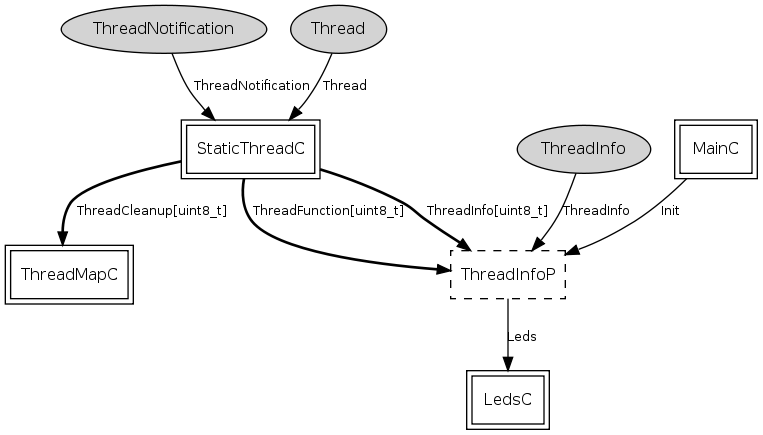
\includegraphics[scale=0.5]{images/tos-lib-tosthreads-system-ThreadC.png}

\paragraph{\textit{chips/atm128/chip\_thread.h}:}
Antes de expor as funções do escalonador de threads, é importante expor algumas macros de baixo nível que realizam a
troca de contexto. Para guardar o contexto de hardware da thread, criaram a estrutura \textit{thread\_regs\_t}.
\begin{lstlisting}
typedef struct thread_regs {
    uint8_t status;
    uint8_t r0;
    ...
    uint8_t r31;
} thread_regs_t;
\end{lstlisting}
Existem também algumas macros para salvar e restaurar estes registradores.
\begin{lstlisting}
 #define SAVE_STATUS(t)                              \
    __asm__("in %0,__SREG__ \n\t" : "=r" ((t)->regs.status) : );

//Save General Purpose Registers
#define SAVE_GPR(t)                                      \
    __asm__("mov %0,r0 \n\t" : "=r" ((t)->regs.r0) : );  \
    ...

//Save stack pointer
#define SAVE_STACK_PTR(t)             \
    __asm__("in %A0, __SP_L__\n\t"    \
    "in %B0, __SP_H__\n\t"            \
    :"=r"((t)->stack_ptr) : );

#define SAVE_TCB(t) \
   SAVE_GPR(t);      \
   SAVE_STATUS(t);   \
   SAVE_STACK_PTR(t) 

//Definicao das macros de restauracao
...

#define SWITCH_CONTEXTS(from, to) \
   SAVE_TCB(from);                 \
   RESTORE_TCB(to)
\end{lstlisting}
Por último, são definidas duas macros para preparação da thread.
%!!!Ainda não descobri para que serve isso exatamente!!!
%O endereço de uma função será colocado no topo da pilha da thread. Pra que ?
%O status é salvo quando SP está apontando para a pilha da thread atual e não para a pilha da que está sendo preparada.
\begin{lstlisting}
 #define SWAP_STACK_PTR(OLD, NEW) \
   __asm__("in %A0, __SP_L__\n\t in %B0, __SP_H__":"=r"(OLD):);\
   __asm__("out __SP_H__,%B0\n\t out __SP_L__,%A0"::"r"(NEW))
 
#define PREPARE_THREAD(t, thread_ptr)                      \
{  uint16_t temp;                                        \
   SWAP_STACK_PTR(temp, (t)->stack_ptr);                 \
   __asm__("push %A0\n push %B0"::"r"(&(thread_ptr)));   \
   SWAP_STACK_PTR((t)->stack_ptr, temp);                 \
   SAVE_STATUS(t)                                        \
}
\end{lstlisting}

\paragraph{\textit{system/TinyThreadSchedulerP.nc}:}
Durante a inicialização do sistema muitas inicializações são feitas através da interface \textit{Init} amarrada ao
compontente \textit{MainC}. Isso ocorre com a \textit{system/StaticThreadP.nc}. Como visto acima, durante a execução
desta função, o escalonador é chamado através do comando a seguir.
\begin{lstlisting}
command error_t ThreadScheduler.initThread(uint8_t id) {
    thread_t* t = (call ThreadInfo.get[id]());
    t->state = TOSTHREAD_STATE_INACTIVE;
    t->init_block = current_thread->init_block;
    call BitArrayUtils.clrArray(t->joinedOnMe, sizeof(t->joinedOnMe));
    PREPARE_THREAD(t, threadWrapper);
        //uint16_t temp;                                        \
        //SWAP_STACK_PTR(temp, (t)->stack_ptr);                 \
        //__asm__("push %A0\n push %B0"::"r"(&(threadWrapper)));   \
        //SWAP_STACK_PTR((t)->stack_ptr, temp);                 \
        //SAVE_STATUS(t)   
    return SUCCESS;
}
\end{lstlisting}
É importante notar que na macro \textit{PREPARE\_THREAD()}, o endereço da função \textit{threadWrapper} está sendo
empilhado na pilha da thread. Está função encapsula a chamada para a execução da thread.
\begin{lstlisting}
void threadWrapper() __attribute__((naked, noinline)) {
    thread_t* t;
    atomic t = current_thread;

    __nesc_enable_interrupt();
    (*(t->start_ptr))(t->start_arg_ptr);

    atomic {
        stop(t);
        sleepWhileIdle();
        scheduleNextThread();
        restoreThread();
    }
}
\end{lstlisting}

No laço principal do escalonador de tarefas, quando não há mais nada para executar, a thread atual é suspensa. Com isso
o controle é passado para o escalonador de threads através do comando \textit{suspendCurrentThread()}. Na demostração de
código abaixo, algumas chamadas a funções são substituídas pelo seus corpos, para facilitar o entendimento.
\begin{lstlisting}
async command error_t ThreadScheduler.suspendCurrentThread() {
    atomic {
        if(current_thread->state == TOSTHREAD_STATE_ACTIVE) {
            current_thread->state = TOSTHREAD_STATE_SUSPENDED;
            //suspend(current_thread);
            #ifdef TOSTHREADS_TIMER_OPTIMIZATION
                num_runnable_threads--;
                post alarmTask();
            #endif
            sleepWhileIdle();
            //interrupt(current_thread);
            yielding_thread = current_thread;
            //scheduleNextThread();
            if(tos_thread->state == TOSTHREAD_STATE_READY)
                current_thread = tos_thread;
            else
                current_thread = call ThreadQueue.dequeue(&ready_queue);

            current_thread->state = TOSTHREAD_STATE_ACTIVE;
            //fim scheduleNextThread();

            if(current_thread != yielding_thread) {
                //switchThreads();
                void switchThreads() __attribute__((noinline)) {
                    SWITCH_CONTEXTS(yielding_thread, current_thread);
                 }
                //fim switchThreads();
            }
            //fim interrupt(...)
            //fim suspend(current_thread);
            return SUCCESS;
        }
        return FAIL;
    }
}
\end{lstlisting}
É muito importante notar que a função \textit{switchThreads()} não é \textit{inline}. Isso significa que os valores dos
registradores serão empilhados. Haverá então uma troca de contexto e o registrador SP apontará para a pilha da nova
thread. Por último, a função \textit{switchThreads()} retornará para o endereço que está no topo da nova pilha. Este
novo endereço, como visto acima, aponta para a função \textit{threadWrapper()}. Esta por sua vez, através de uma função
e duas sinalizações executa a thread.

\paragraph{Trocas de Contextos}
acontecem por três motivos diferentes: ocorrência de uma interrupção, termino do tempo de execução da thread, ou chamadas
bloqueantes ao sistema. 
Para implementar o primeiro caso, é inserida a função \textit{postAmble} ao final de todas as rotinas de processamento
de interrupção. Esta função verifica se foi postada uma nova tarefa, e caso positivo, o controle é passado para o
\textit{kernel}. Caso contrário, a thread continua a executar logo após o termino do tratador de interrupção.
Para implementar o segundo caso, é utilizado um temporizador que provoca uma interrupção ao final de cada
\textit{timeslice}. Esta posta uma tarefa, forçando o \textit{kernel} a assumir o controle e escalonar a próxima thread.
%!!!Botar código?!!!

As chamadas de sistema transformam os serviços de duas fases dos TinyOS em chamadas bloqueantes. Para o programador isso
facilita a programação pois torna o fluxo do código continuo. Para permitir isto, essa nova estrutura posta uma tarefa
que executará a primeira fase do serviço (\textit{command}/\textit{call}), suspende a thread e a acorda o
\textit{kernel} para escalonar outra thread. Ao chegar o evento (através de uma tarefa), a \textit{syscall} acorda a thread e lhe repassa o dado.
%!!! Botar código? !!!
